% =====================================================================
% NeuroQuest -- IEEE conference paper (IEEEtran). Compile with pdfLaTeX
% (e.g. upload this folder to Overleaf). Items marked TODO need the authors.
% =====================================================================
\documentclass[conference]{IEEEtran}
\IEEEoverridecommandlockouts
\usepackage{cite}
\usepackage{amsmath,amssymb,amsfonts}
\usepackage{graphicx}
\usepackage{booktabs}
\usepackage{multirow}
\usepackage{xcolor}
\usepackage{url}
\usepackage{tikz}
\usetikzlibrary{positioning,arrows.meta,fit,backgrounds}
\graphicspath{{figures/}}

\begin{document}

\title{NeuroQuest: Explainable Multimodal Fusion for Game-Based Screening of Dyslexia, Dysgraphia and Dyscalculia with Safe Continual Retraining}

% TODO: authors and affiliations
\author{\IEEEauthorblockN{Author One}
\IEEEauthorblockA{\textit{Department} \\ \textit{University}\\ City, Country \\ email}
\and
\IEEEauthorblockN{Author Two}
\IEEEauthorblockA{\textit{Department} \\ \textit{University}\\ City, Country \\ email}
}

\maketitle

% ---------------------------------------------------------------------
\begin{abstract}
Specific learning disorders such as dyslexia, dysgraphia and dyscalculia are often identified late, after years of
academic difficulty. Game-based screening can reach children early, but most published systems score a single kind of
evidence with a single model, report accuracy on one train--test split, and offer no explanation or path to improve once
deployed. We present NeuroQuest, an end-to-end screening system that couples a child-friendly assessment game with an
explainable multimodal machine-learning pipeline. For each disorder we organise the available evidence into
modalities (task accuracy, interaction behaviour, response time, handwriting geometry, deep visual features and
number-sense measures) and compare unimodal baselines with early, late and hybrid fusion under nested
cross-validation. Fusion improved ROC-AUC for dyslexia from 0.804 to 0.862 (balanced accuracy 0.778, sensitivity
0.811) on 5,039 children, and reached 0.933 for dysgraphia on 249 handwriting samples. On a small real dyscalculia
cohort ($n=37$), fusion gave no benefit. SHAP and occlusion analyses explain predictions at three levels: modality,
feature or game question, and individual child. We also report data-quality problems that would otherwise inflate
results, including a resolution confound in handwriting scans and label-leaking variables. The trained models are
deployed behind the game through a scoring service with rule-based fallback. A champion--challenger loop retrains on
specialist-confirmed game sessions and promotes a new model only when it outperforms the live one on unseen children.
\end{abstract}

\begin{IEEEkeywords}
dyslexia, dysgraphia, dyscalculia, multimodal fusion, explainable AI, SHAP, serious games, nested cross-validation, continual learning
\end{IEEEkeywords}

% ---------------------------------------------------------------------
\section{Introduction}
Specific learning disorders (SLDs) affect an estimated 5--15\% of school-age children and include impairments in
reading (dyslexia), written expression (dysgraphia) and mathematics (dyscalculia). Early identification enables
targeted intervention, but formal assessment by psychologists is costly and often happens only after sustained
failure. Gamified screening offers a scalable alternative: children play short tasks while the system records how
they perform.

Existing AI-based screening work has three recurring limitations
\cite{bhushan2024survey,fallah2025dysgraphia}. (i)~Most systems use one data modality, such as only answer
correctness or only handwriting images, and one classifier. (ii)~Many studies report plain accuracy on a single
split. On imbalanced screening data this is misleading: in the dyslexia data used here, always predicting ``no risk''
already scores 89.3\%. (iii)~Models are rarely explained and almost never deployed with a mechanism to keep improving
on the target population.

This paper presents NeuroQuest, which addresses these gaps. Our contributions are:
\begin{enumerate}
  \item A \textbf{systematic comparison of fusion strategies}: unimodal, early, late (three combiners) and hybrid fusion,
        evaluated identically for three disorders on four datasets.
  \item A \textbf{leakage-free evaluation protocol}. Nested cross-validation selects per-modality algorithms, fusion
        weights, meta-learners and decision thresholds without touching test folds. A ``simplest model within noise''
        rule then picks the deployed model.
  \item \textbf{Data-quality findings} that change conclusions: corrupted ratio fields, a scan-resolution shortcut in
        handwriting images, and label-leaking variables.
  \item \textbf{Three-level explainability}: modality importance, feature and game-question attribution, and
        per-child explanations including handwriting occlusion maps.
  \item A \textbf{deployed system with safe continual retraining}. A scoring service with rule-based fallback, minimal
        game extensions that collect model-ready inputs, and a champion--challenger loop driven by specialist-confirmed
        outcomes.
\end{enumerate}

% ---------------------------------------------------------------------
\section{Related Work}
\textit{Game-based dyslexia screening.} Rello \emph{et al.}~\cite{rello2020dyt} showed that interaction data from a
32-question online gamified test (Dytective) can predict dyslexia risk. Their released desktop and tablet datasets
are used here. We extend that line of work by treating accuracy, interaction behaviour and demographics as
separate modalities and quantifying the benefit of fusing them.

\textit{Dysgraphia.} A recent scoping review~\cite{fallah2025dysgraphia} groups approaches into online kinematic
methods (tablet strokes) and offline image-based methods (scanned handwriting), using hand-crafted features or CNNs.
Few studies combine both feature families or examine acquisition confounds. We combine interpretable geometry
features with CNN embeddings and explicitly control for scan resolution.

\textit{Dyscalculia.} AI-based dyscalculia screening remains sparse and data-poor~\cite{bhushan2024survey}.
Cognitive studies identify impaired approximate number system (ANS) acuity~\cite{piazza2010acuity}, immature
number-line mappings~\cite{siegler2003numberline} and largely intact subitizing~\cite{decarli2020subitizing} as
markers. We use these findings to design game tasks and to build a simulation for testing the pipeline.

\textit{Multimodal fusion and XAI.} Fusion is commonly grouped into early (feature-level), late (decision-level) and
hybrid schemes~\cite{baltrusaitis2019multimodal}. We explain predictions with SHAP~\cite{lundberg2017shap} and
occlusion sensitivity~\cite{zeiler2014visualizing}. Because model selection inside a cross-validation loop biases
error estimates~\cite{varma2006bias}, we use nested cross-validation throughout.

% ---------------------------------------------------------------------
\section{Datasets}
Table~\ref{tab:data} summarises the data.

\textbf{Dyslexia (Dyt)}~\cite{rello2020dyt}. 3,644 desktop and 1,395 tablet participants aged 7--17, with 10.7\%
labelled at risk. For each of 32 questions the data records clicks, hits, misses, score, accuracy and miss rate, plus
gender, language flags and age. About 5,000 \emph{Accuracy} and \emph{Missrate} cells had lost their decimal point
(e.g.\ 0.875 stored as 875), so we recomputed them as \emph{Hits}/\emph{Clicks} and \emph{Misses}/\emph{Clicks}.
These identities hold for 99\% of clean cells. Question 29 was never shown on tablets and was removed. Other
tablet gaps are imputed inside each training fold, with missing-value indicators.

\textbf{Dysgraphia.} 249 binarised scans of children copying a short sentence, labelled \emph{potential}
(114) or \emph{low-potential} (135) dysgraphia~\cite{dysgraphiadata}. % TODO: confirm dataset citation

\textbf{Dyscalculia (real).} The Castaldi \emph{et al.} time-perception dataset~\cite{castaldi2024data}: 37 children
(15 with developmental dyscalculia), with time-perception precision (Weber fraction) and point of subjective equality
at 500\,ms and 1500\,ms, age, non-verbal IQ and gender. We exclude the \emph{math} index because it is the
diagnostic criterion. We also exclude \emph{reading}, which is 46\% missing and whose values and missingness both
separate the groups.

\textbf{Dyscalculia (synthetic).} No public dataset matches our game's number tasks, so we simulate 3,000 children
playing extended versions of them (Section~\ref{sec:synthetic}). This data is used only to test the pipeline and the
explanations; its scores are never reported as clinical performance.

\begin{table}[t]
\caption{Datasets and modalities}
\label{tab:data}
\centering
\footnotesize
\setlength{\tabcolsep}{3pt}
\begin{tabular}{@{}lrrl@{}}
\toprule
Dataset & $n$ & Pos. & Modalities (features) \\
\midrule
Dyslexia (Dyt) & 5,039 & 540 & Demographics (5), Task accuracy (93), \\
 & & & Interaction behaviour (93) \\
Dysgraphia & 249 & 114 & Handwriting geometry (25), \\
 & & & Deep visual, EfficientNet-B0 (1,280) \\
Dyscalc.\ (real) & 37 & 15 & Time perception (4), Cognitive profile (3) \\
Dyscalc.\ (synth.) & 3,000 & 401 & Demographics (2), Accuracy (6), \\
 & & & Response time (11), Number sense (8) \\
\bottomrule
\end{tabular}
\end{table}

% ---------------------------------------------------------------------
\section{Proposed System}

\subsection{Architecture}
Fig.~\ref{fig:arch} shows the system. A React web game delivers 17 tasks: five per disorder, plus two new tasks
described in Section~\ref{sec:deploy}. A Spring Boot backend stores sessions in MongoDB and computes the existing
rule-based report. A Python (FastAPI) ML service then scores the session with the active model for each disorder.
Its results are attached to the report, and a model trained on real data overrides the rule-based risk level for its
disorder. An offline research pipeline trains and evaluates all fusion variants. A model registry tracks versions,
and a retraining job closes the loop using specialist-confirmed outcomes.

\begin{figure*}[t]
\centering
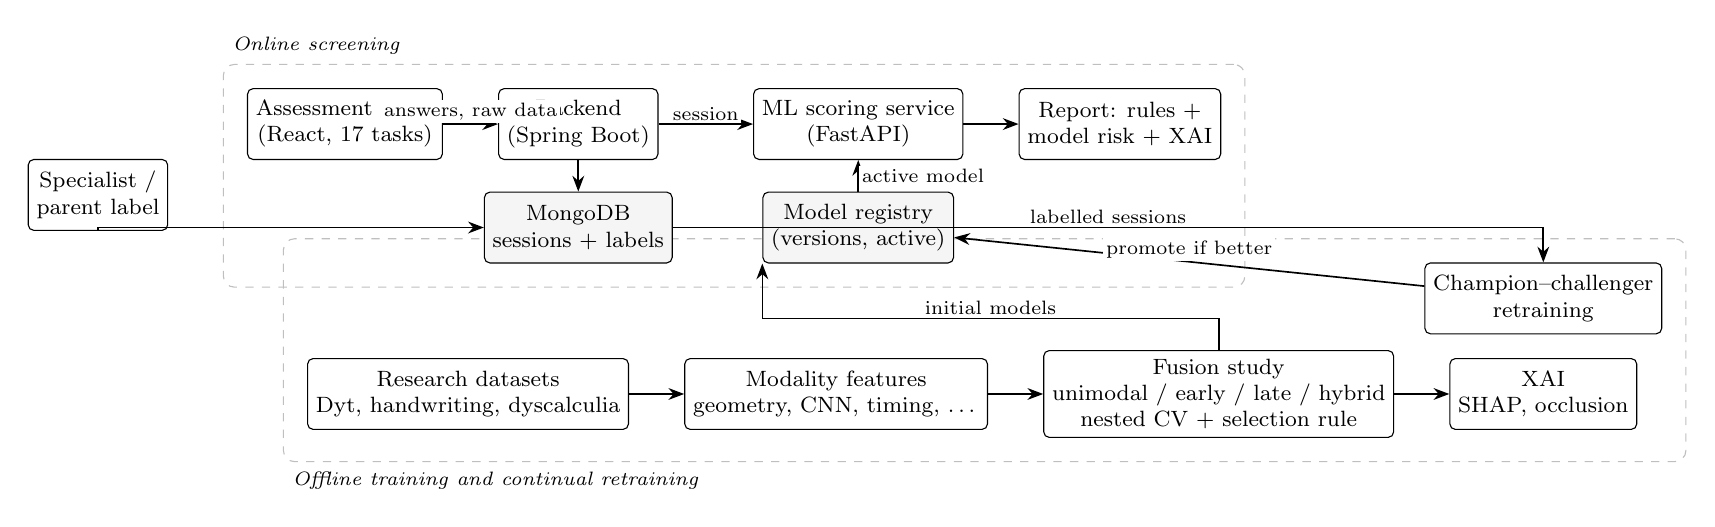
\begin{tikzpicture}[
  node distance=4mm and 7mm,
  box/.style={draw, rounded corners=2pt, align=center, font=\footnotesize, minimum height=9mm, inner sep=3pt, fill=white},
  store/.style={box, fill=gray!8},
  arr/.style={-{Stealth[length=2mm]}, semithick},
  lab/.style={font=\scriptsize, fill=white, inner sep=1pt}]
  % row 1: online path
  \node[box] (game) {Assessment game\\(React, 17 tasks)};
  \node[box, right=of game] (be) {Backend\\(Spring Boot)};
  \node[store, below=of be] (db) {MongoDB\\sessions + labels};
  \node[box, right=12mm of be] (ml) {ML scoring service\\(FastAPI)};
  \node[box, right=of ml] (rep) {Report: rules +\\model risk + XAI};
  \node[store, below=of ml] (reg) {Model registry\\(versions, active)};
  % row 3: offline research + retraining
  \node[box, below=12mm of db, xshift=-14mm] (data) {Research datasets\\Dyt, handwriting, dyscalculia};
  \node[box, right=of data] (fe) {Modality features\\geometry, CNN, timing, \dots};
  \node[box, right=of fe] (fus) {Fusion study\\unimodal / early / late / hybrid\\nested CV + selection rule};
  \node[box, right=of fus] (xai) {XAI\\SHAP, occlusion};
  \node[box, above=of xai, yshift=-1mm] (rt) {Champion--challenger\\retraining};
  \node[box, left=10mm of game, yshift=-9mm] (sp) {Specialist /\\parent label};

  \draw[arr] (game) -- node[lab, above]{answers, raw data} (be);
  \draw[arr] (be) -- (db);
  \draw[arr] (be) -- node[lab, above]{session} (ml);
  \draw[arr] (ml) -- (rep);
  \draw[arr] (reg) -- node[lab, right]{active model} (ml);
  \draw[arr] (sp) |- (db);
  \draw[arr] (db) -| node[lab, pos=0.25, above]{labelled sessions} (rt);
  \draw[arr] (rt) -- node[lab, above]{promote if better} (reg);
  \draw[arr] (data) -- (fe);
  \draw[arr] (fe) -- (fus);
  \draw[arr] (fus) -- (xai);
  \draw[arr] (fus.north) -- ++(0,4mm) -| node[lab, pos=0.25, above]{initial models} (reg.south west);
  \begin{scope}[on background layer]
    \node[draw=gray!50, dashed, rounded corners, fit=(game)(be)(db)(ml)(rep)(reg), inner sep=3mm,
          label={[font=\scriptsize\itshape, anchor=south west]north west:Online screening}] {};
    \node[draw=gray!50, dashed, rounded corners, fit=(data)(fe)(fus)(xai)(rt), inner sep=3mm,
          label={[font=\scriptsize\itshape, anchor=north west]south west:Offline training and continual retraining}] {};
  \end{scope}
\end{tikzpicture}
\caption{NeuroQuest architecture. The online path scores each session with the active model per disorder and falls
back to rules when no model applies. The offline path trains and explains the fusion models, and retrains from
confirmed outcomes under a champion--challenger policy.}
\label{fig:arch}
\end{figure*}

\subsection{Modality Construction}
\textit{Dyslexia.} The 186 per-question features are split by what they measure. \emph{Task accuracy} covers hits,
score and accuracy. \emph{Interaction behaviour} covers clicks, misses and miss rate, which reflect impulsive or
hesitant interaction. \emph{Demographics} is the third modality.

\textit{Dysgraphia.} Preprocessing has four steps. Images are Otsu-binarised. Ruled lines are found with a long
horizontal morphological opening and subtracted. Strokes cut by a line are rejoined by a vertical closing sized to
the measured line thickness. Finally, the image is \emph{rescaled so the median letter height is 40\,px}.

This last step matters: raw letter height in pixels alone separates the classes with AUC 0.90, but scan resolution
is unknown. A model could therefore learn the scanner rather than the handwriting.

From the normalised image we compute 25 \emph{geometry} features. They cover letter-size variability, baseline and
top-line residuals, spacing statistics, slant mean and variability, relative stroke width and its variability,
contour convexity, a contour-tremor index and stroke fragmentation, all expressed in letter-height units. The
\emph{deep visual} modality averages EfficientNet-B0~\cite{tan2019efficientnet} embeddings over overlapping
224$\times$224 tiles of the strip. It is reduced by PCA to 32 components inside each training fold.

\textit{Dyscalculia.} The real data has two modalities: time perception and cognitive profile. Game trial logs are
turned into accuracy, response-time and number-sense features. The number-sense features are a maximum-likelihood
ANS Weber fraction, the ratio effect, number-line percent absolute error, linear versus logarithmic fit, subitizing
span and error.

\subsection{Fusion Strategies}
Let $\mathbf{x}^{(m)}$ be the features of modality $m\in\{1,\dots,M\}$.
\begin{itemize}
  \item \textbf{Unimodal}: $p_m=f_m(\mathbf{x}^{(m)})$ for each modality and algorithm. This is the baseline.
  \item \textbf{Early fusion}: $p=f([\mathbf{x}^{(1)};\dots;\mathbf{x}^{(M)}])$ with logistic regression, random forest,
        XGBoost~\cite{chen2016xgboost}, MLP or SVM. Per-modality preprocessing, such as PCA for CNN features, is applied first.
  \item \textbf{Late fusion}: the best algorithm per modality, chosen on inner out-of-fold AUC, produces $p_m$. These are combined by
        (a) soft voting $\bar p=\frac1M\sum_m p_m$; (b) AUC-weighted voting with $w_m\propto\max(\mathrm{AUC}_m-0.5,\epsilon)$;
        or (c) stacking, a logistic-regression meta-learner on $\mathrm{logit}(p_m)$ trained on out-of-fold predictions.
  \item \textbf{Hybrid fusion}: a stacking meta-learner over $\{\mathrm{logit}(p_m)\}$ and the logit of the best early-fusion model.
\end{itemize}
Class imbalance is handled with class weights. The decision threshold of every model is the one that maximises
balanced accuracy (Youden's $J$) on training-side out-of-fold predictions.

\subsection{Evaluation Protocol and Model Selection}
All results use \emph{nested} stratified cross-validation. Dyslexia uses 5 outer folds, dysgraphia 5 folds
$\times$ 3 repeats, and real dyscalculia 5 folds $\times$ 10 repeats; inner loops use 3--5 folds. Every
label-dependent choice is made inside the outer training split: imputation, scaling, PCA, per-modality algorithm,
fusion weights, meta-learner and threshold.

We report ROC-AUC, balanced accuracy, sensitivity, specificity, F1 and PR-AUC as mean $\pm$ s.d.\ over outer test
folds. Where each sample is predicted once, we also give a bootstrap 95\% CI. For deployment we do not simply take
the top scorer. Among all models within 0.005 ROC-AUC of the best, we pick the \emph{simplest}, ordering by fewer
stages first and then by the simpler algorithm.

\subsection{Explainability}
Explanations are produced at three levels.
\begin{itemize}
  \item \emph{Modality level}: the share of total $|\mathrm{SHAP}|$ per modality, and grouped permutation importance
        (the drop in held-out AUC when all of a modality's columns are shuffled together).
  \item \emph{Feature and question level}: TreeSHAP for XGBoost and permutation SHAP otherwise. For dyslexia, SHAP is
        summed over each question's features to rank the game's questions.
  \item \emph{Individual level}: SHAP waterfalls, per-modality log-odds contributions from the stacking meta-learner,
        and occlusion maps on held-out handwriting.
\end{itemize}

\subsection{Synthetic Game Telemetry}\label{sec:synthetic}
Each simulated child has correlated latent abilities: ANS acuity, symbolic and arithmetic skill, speed, attention
and subitizing. Children with dyscalculia are shifted by $-1.4$ SD (arithmetic), $-1.0$ (ANS), $-0.3$ (speed and
subitizing) and $-0.2$ (attention), following~\cite{piazza2010acuity,decarli2020subitizing}.

The simulation also includes age-dependent development, namely ANS sharpening and the logarithmic-to-linear
number-line shift~\cite{siegler2003numberline}. Eight percent of non-dyscalculic children are given attention
difficulties as confounders, and 5\% of labels are flipped.

Trials are generated for the game's five tasks: 10 subitizing, 16 magnitude-comparison, 10 number-line (0--20),
6 sequence and 10 addition trials. Because the generator is known, the data also tests the explanations: a correct
explainer must rank arithmetic features first and subitizing last.

\subsection{Deployment and Continual Retraining}\label{sec:deploy}
To keep game changes small, we add only two tasks.
\begin{itemize}
  \item \emph{Copy the sentence}: a free-handwriting canvas exported as an image, with stroke jitter and hesitation
        measured from the pen trajectory. Previously this score was a constant.
  \item \emph{Number-sense round}: repeated short trials logged in the model's input format.
\end{itemize}

The scoring service returns, per disorder, a probability and a risk level. MODERATE starts at the selected
threshold, and HIGH starts where 95\% of true negatives score lower. Each result also carries per-modality
contributions. A model trained on synthetic data is displayed but never changes the report.

Specialists confirm outcomes after assessment, and parents may report prior diagnoses as weaker labels. After every
20 new labels for a disorder, the service retrains on game data with the same fusion pipeline. The challenger is
promoted only if it (i) clears AUC 0.65 and (ii) beats the champion by at least 0.01 AUC. The champion's score is
measured on labelled sessions \emph{it was not trained on}. All versions are retained for audit and rollback.

% ---------------------------------------------------------------------
\section{Results}

\subsection{Effect of Fusion}
Table~\ref{tab:fusion} reports the best model of each family.

\textbf{Dyslexia.} Fusion was clearly beneficial. The best single modality, interaction behaviour with XGBoost,
reached 0.804 ROC-AUC. Early fusion reached 0.862 (+0.058) and late fusion 0.846 (+0.042). Hybrid fusion scored
0.863, but its edge over early fusion (0.001) is far inside the fold s.d.\ ($\pm$0.020), so the selection rule
deploys early-fusion XGBoost.

The deployed model has balanced accuracy 0.778, sensitivity 0.811 and specificity 0.745. Its pooled out-of-fold AUC
is 0.861 (bootstrap 95\% CI 0.845--0.876). Performance was higher on desktop (AUC 0.883) than on tablet (0.797), where several
questions are partly or entirely missing.

\textbf{Dysgraphia.} Early fusion with logistic regression achieved 0.933 $\pm$ 0.034 ROC-AUC and 0.850 balanced
accuracy (sensitivity 0.863, specificity 0.837). That is +0.013 over the best single modality, the CNN features
alone at 0.920. Late fusion added only 0.003. Both modalities look at the same image, which explains the small
gain.

\textbf{Dyscalculia.} On the real cohort, time perception alone reached 0.765. Early fusion matched it (0.766), and
late and hybrid fusion were \emph{worse} (0.696 and 0.697). With 37 children the stacking combiner overfits, and the
cognitive-profile modality carries no signal (AUC $\approx$ 0.5). On synthetic data every fusion type gained about
+0.01 over response time alone (0.731). The best model's AUC of 0.742 compares with a ceiling of 0.847 implied by the
label noise.

\begin{table}[t]
\caption{Best model per fusion family: ROC-AUC (mean $\pm$ s.d.\ over outer folds) and balanced accuracy. Bold marks the deployed model.}
\label{tab:fusion}
\centering
\footnotesize
\setlength{\tabcolsep}{2.5pt}
\begin{tabular}{@{}llcc@{}}
\toprule
Dataset & Family (best model) & ROC-AUC & Bal.\ acc. \\
\midrule
\multirow{4}{*}{Dyslexia} & Unimodal (interaction, XGB) & 0.804 $\pm$ .039 & 0.734 \\
 & \textbf{Early (XGBoost)} & \textbf{0.862 $\pm$ .023} & \textbf{0.778} \\
 & Late (soft voting) & 0.846 $\pm$ .026 & 0.761 \\
 & Hybrid & 0.863 $\pm$ .020 & 0.769 \\
\midrule
\multirow{4}{*}{Dysgraphia} & Unimodal (CNN, LR) & 0.920 $\pm$ .042 & 0.831 \\
 & \textbf{Early (LR)} & \textbf{0.933 $\pm$ .034} & \textbf{0.850} \\
 & Late (AUC-weighted) & 0.923 $\pm$ .041 & 0.847 \\
 & Hybrid & 0.923 $\pm$ .041 & 0.840 \\
\midrule
\multirow{4}{*}{Dyscalc.\ (real)} & \textbf{Unimodal (time perc., LR)} & \textbf{0.765 $\pm$ .174} & \textbf{0.679} \\
 & Early (RF) & 0.766 $\pm$ .162 & 0.650 \\
 & Late (AUC-weighted) & 0.696 $\pm$ .211 & 0.632 \\
 & Hybrid & 0.697 $\pm$ .194 & 0.616 \\
\midrule
\multirow{4}{*}{Dyscalc.\ (synth.)} & Unimodal (resp.\ time, LR) & 0.731 $\pm$ .008 & 0.671 \\
 & \textbf{Early (LR)} & \textbf{0.741 $\pm$ .020} & \textbf{0.688} \\
 & Late (AUC-weighted) & 0.741 $\pm$ .020 & 0.673 \\
 & Hybrid & 0.739 $\pm$ .016 & 0.683 \\
\bottomrule
\end{tabular}
\end{table}

\begin{figure}[t]
\centering
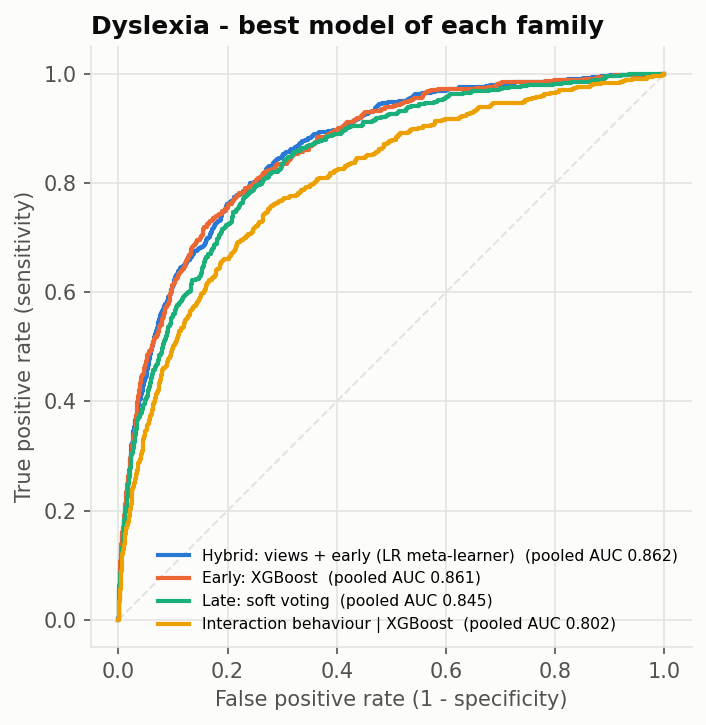
\includegraphics[width=0.92\columnwidth]{dyslexia_roc.png}
\caption{Dyslexia: pooled out-of-fold ROC curves of the best model in each family.}
\label{fig:roc}
\end{figure}

\subsection{Explainability Findings}
\textbf{Dyslexia.} Interaction behaviour accounted for 42.6\% of total $|\mathrm{SHAP}|$, task accuracy for 35.3\%
and demographics for 22.1\% (Fig.~\ref{fig:shap}). The most influential features were native-language status, age,
and click counts on questions 28, 24 and 25.

Aggregated by question, items Q24, Q28, Q25, Q20 and Q22 contributed most. This ranking is directly usable for
redesigning the game: keep and extend the informative items, and shorten the rest. The strong weight on language and
age is likely a property of how this cohort was collected, and should be re-checked on game data.

\begin{figure}[t]
\centering
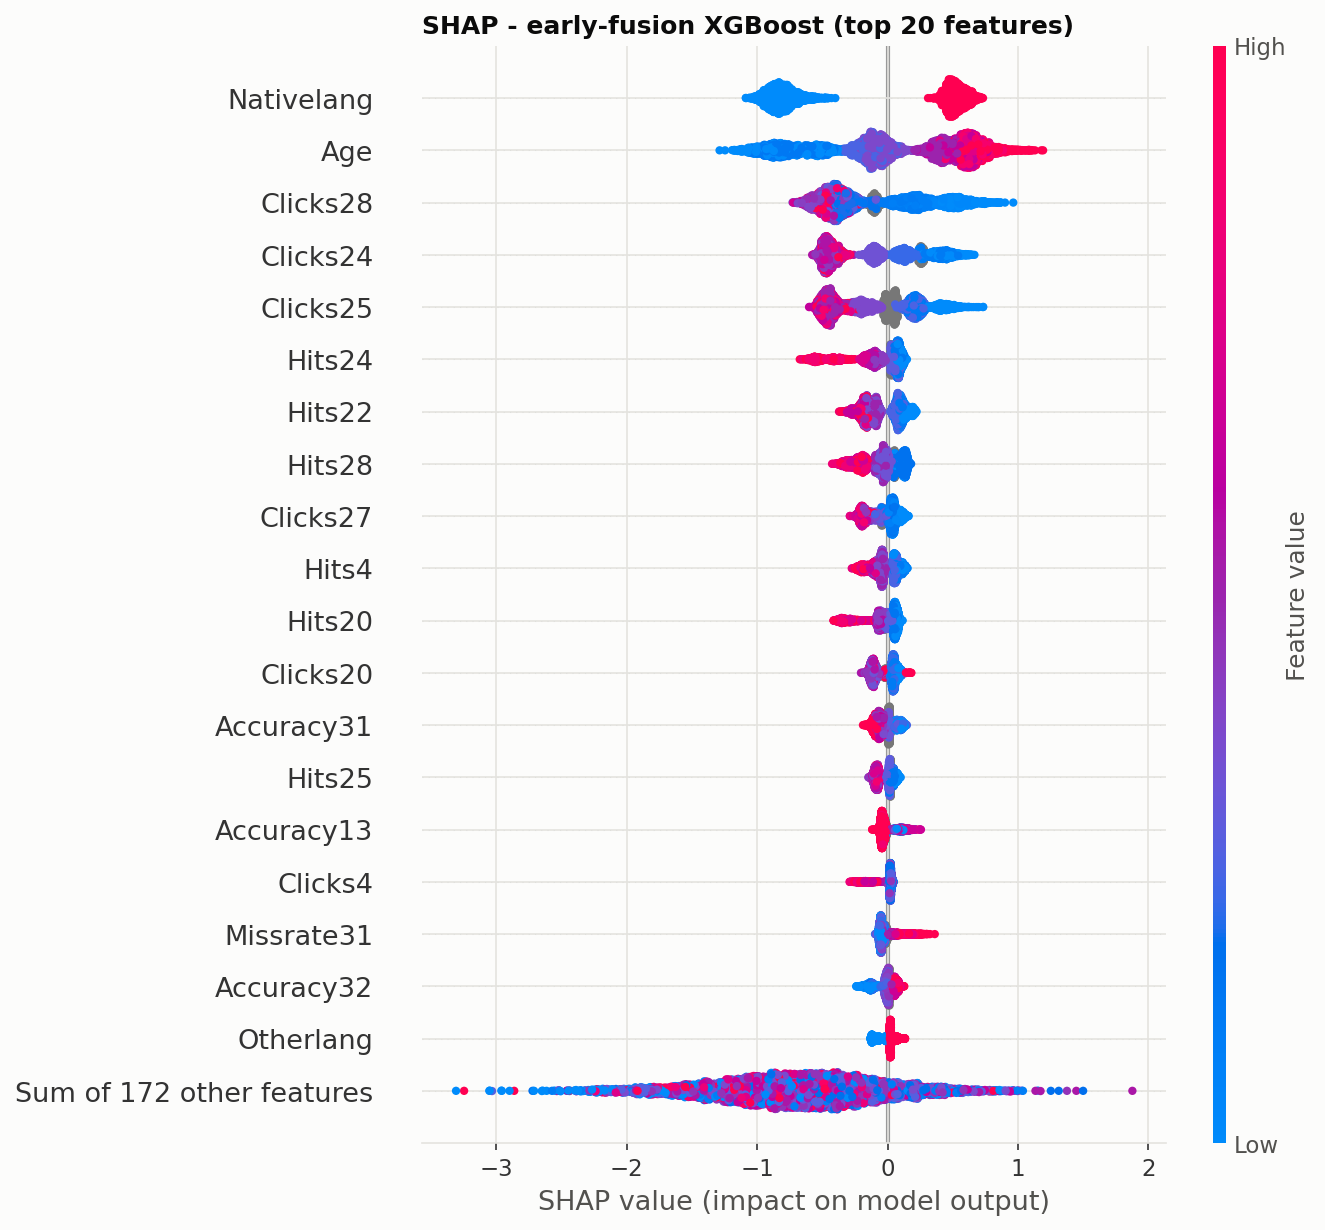
\includegraphics[width=0.95\columnwidth]{dyslexia_shap.png}
\caption{SHAP summary of the early-fusion XGBoost dyslexia model (top 20 features).}
\label{fig:shap}
\end{figure}

\textbf{Dysgraphia.} Grouped permutation importance shows the CNN modality dominates. Shuffling it lowered held-out
AUC by 0.340, against 0.041 for the geometry modality. Among geometry features, the most influential were the
spread of letter heights, gap variability, sentence length in letter heights, contour convexity and stroke
fragmentation. Higher fragmentation (broken strokes) increased risk.

Two findings call for caution. More \emph{regular} spacing was associated with risk, and occlusion maps
(Fig.~\ref{fig:occl}) highlight stroke regions whose thickness differs visibly between classes. Part of the 0.933
AUC may therefore reflect pen or acquisition differences between groups rather than handwriting quality.

\begin{figure}[t]
\centering
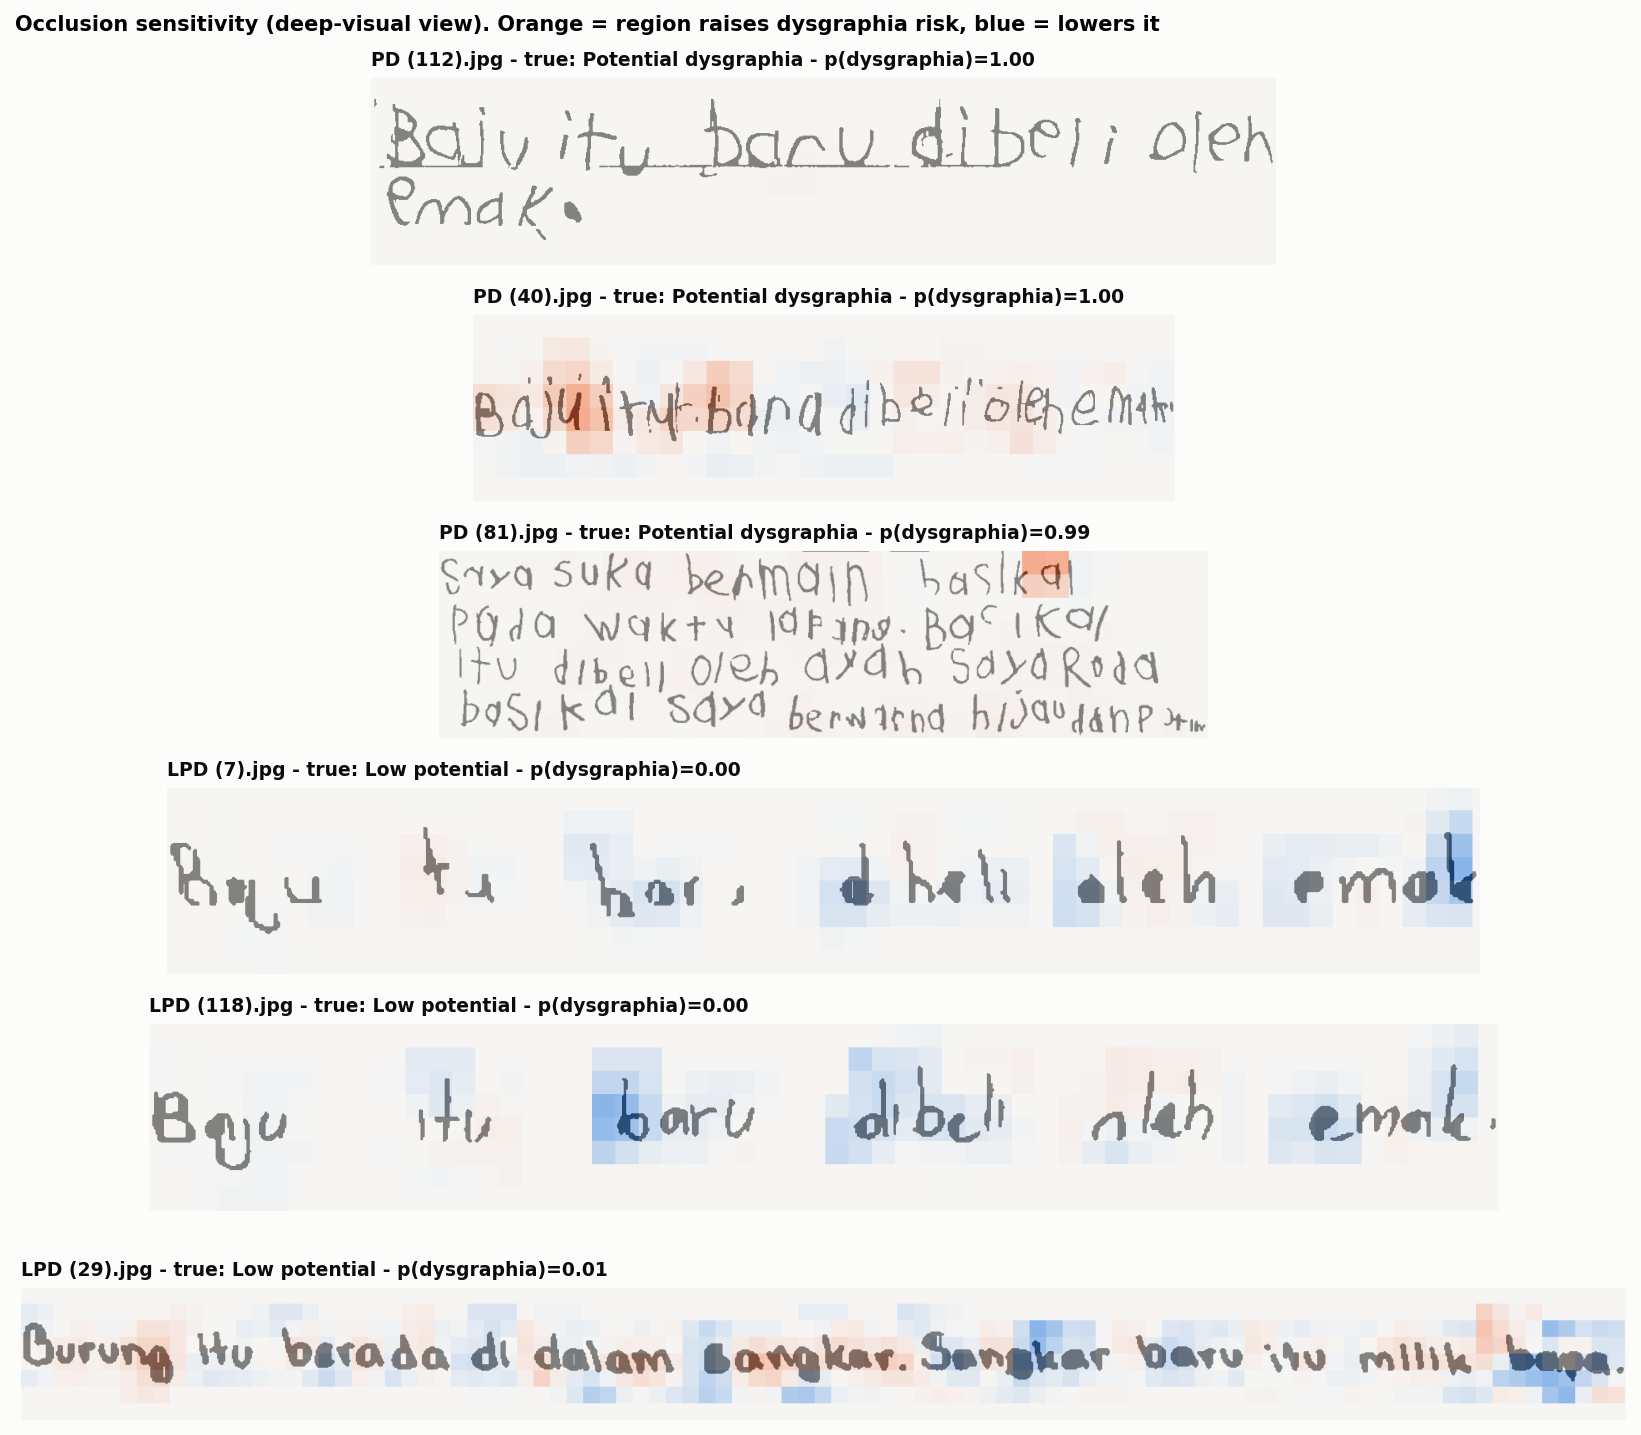
\includegraphics[width=\columnwidth]{dysgraphia_occlusion.png}
\caption{Occlusion sensitivity on held-out handwriting (CNN modality). Orange regions raise the predicted dysgraphia risk; blue regions lower it.}
\label{fig:occl}
\end{figure}

\textbf{Dyscalculia.} On real data, time-perception precision (Weber fraction at 500\,ms and 1500\,ms) was most
informative, with higher Weber fractions associated with dyscalculia. This is consistent with the source
study~\cite{castaldi2024data}.

On synthetic data the explanations recovered the planted structure. Arithmetic and sequence response time and
arithmetic accuracy ranked first, number-line error and linearity followed, and subitizing ranked last. This is a
sanity check that the XAI layer reflects real model behaviour.

\subsection{Data-Quality Effects}
Three issues would have inflated or distorted results if left untreated.
\begin{itemize}
  \item Without scale normalisation, a single resolution-dependent feature reached AUC 0.92 for dysgraphia.
  \item In the real dyscalculia data, \emph{math} and \emph{reading} each separate the classes perfectly.
  \item Corrupted ratio fields in Dyt would have introduced values two to three orders of magnitude too large.
\end{itemize}

\subsection{Deployed System}
Table~\ref{tab:deploy} lists the models deployed at launch. The dyslexia model needs the 32 Dyt questions, which the
game does not contain, so dyslexia uses rule-based scoring until enough labelled game sessions allow a game-native
model.

In an end-to-end test through the production APIs, a session with a handwriting sample and a number-sense round was
scored by both models, and the real-data dysgraphia model set the report's risk level. On 160 simulated game
sessions, the retraining loop behaved as intended. The first run trained game-native models and promoted them. The
second run kept the live models, because no challenger beat them by the required margin on unseen sessions.

\begin{table}[t]
\caption{Models deployed in the game at launch}
\label{tab:deploy}
\centering
\footnotesize
\setlength{\tabcolsep}{3pt}
\begin{tabular}{@{}llll@{}}
\toprule
Disorder & Model (input) & AUC & Role \\
\midrule
Dyslexia & Rules (game Q1--Q5) & -- & Until labelled data \\
Dysgraphia & Early fusion LR (Q16 image) & 0.933 & Sets risk \\
Dyscalculia & Early fusion LR (Q17 trials) & 0.741$^\dagger$ & Display only \\
\bottomrule
\multicolumn{4}{@{}l}{\scriptsize $^\dagger$ trained and evaluated on synthetic data; not a clinical estimate.}
\end{tabular}
\end{table}

% ---------------------------------------------------------------------
\section{Discussion}
\textit{When does fusion help?} Fusion paid off when modalities captured \emph{different} aspects of behaviour, as
with what a child answered versus how they clicked in dyslexia. Early fusion was best because it can model
cross-modal interactions. Gains were small when modalities were different views of the same signal (handwriting
geometry versus CNN). Late fusion was harmful when one modality was uninformative and the sample tiny (real
dyscalculia). Practitioners should therefore report unimodal baselines and per-modality importance rather than
assuming fusion is always better.

\textit{Why rigorous evaluation matters.} Several of our intermediate results would have looked much better under a
naive protocol: plain accuracy of 0.89 for a useless dyslexia model, near-perfect separation from leaked variables,
and resolution shortcuts in images. Nested cross-validation, imbalance-aware metrics and explicit confound checks
were necessary to obtain trustworthy estimates.

\textit{Limitations.}
\begin{itemize}
  \item No child appears in more than one dataset, so disorders are fused \emph{within} but not \emph{across}.
  \item The dysgraphia dataset is small and may contain acquisition confounds. The model was trained on paper
        scans, while the game collects on-screen handwriting.
  \item The real dyscalculia cohort is very small, and the deployed dyscalculia model is a placeholder trained on
        synthetic data.
  \item Labels are screening-level, not necessarily formal diagnoses.
\end{itemize}
The retraining loop was validated only on simulated sessions; its real benefit depends on the volume and quality of
confirmed labels.

\textit{Ethics.} The system is a screening aid, not a diagnostic tool. Handwriting samples and outcome labels are
sensitive data about children, so deployment requires informed consent, authenticated access to labelling and
training endpoints, and a data-retention policy.

% ---------------------------------------------------------------------
\section{Conclusion and Future Work}
We presented NeuroQuest, an explainable multimodal screening system for dyslexia, dysgraphia and dyscalculia.
Under nested cross-validation, early fusion improved dyslexia screening from 0.804 to 0.862 ROC-AUC and reached
0.933 for dysgraphia, while explanations exposed which modalities, game questions and handwriting regions drive each
decision. The models run behind the game with rule-based fallback, and a champion--challenger loop allows safe
improvement from confirmed outcomes.

Future work includes:
\begin{itemize}
  \item collecting labelled sessions from the game to train game-native models and to validate the handwriting model
        on screen input;
  \item extending the number-sense round to a validated dyscalculia battery;
  \item a cross-disorder model trained on children who complete all tasks;
  \item studying fairness across age, language and device.
\end{itemize}

% ---------------------------------------------------------------------
% TODO: verify every reference against the original source before submission.
\begin{thebibliography}{99}

\bibitem{rello2020dyt}
L.~Rello, R.~Baeza-Yates, A.~Ali, J.~P.~Bigham, and M.~Serra, ``Predicting risk of dyslexia with an online gamified test,'' \emph{PLoS ONE}, vol.~15, no.~12, e0241687, 2020.

\bibitem{bhushan2024survey}
S.~Bhushan, S.~Arunkumar, T.~A.~E.~Eisa, M.~Nasser, A.~K.~Singh, and P.~Kumar, ``AI-enhanced dyscalculia screening: A survey of methods and applications for children,'' \emph{Diagnostics}, vol.~14, no.~13, p.~1441, 2024.

\bibitem{fallah2025dysgraphia}
A.~Fallah, Y.~ZandiyeVakili, and H.~Sajedi, ``AI-driven approaches for dysgraphia diagnosis using online and offline handwriting data: A comprehensive scoping review,'' \emph{PLoS ONE}, vol.~20, no.~12, e0328722, 2025.

\bibitem{dysgraphiadata}
% TODO: replace with the source of the dysgraphia handwriting dataset used in datasets/DATASET DYSGRAPHIA HANDWRITING
``Dysgraphia handwriting dataset (potential vs.\ low-potential dysgraphia),'' [Online]. Available: TODO.

\bibitem{castaldi2024data}
E.~Castaldi \emph{et al.}, ``Auditory time perception impairment in children with developmental dyscalculia,'' dataset, Zenodo, record 10966052, 2024.

\bibitem{piazza2010acuity}
M.~Piazza \emph{et al.}, ``Developmental trajectory of number acuity reveals a severe impairment in developmental dyscalculia,'' \emph{Cognition}, vol.~116, no.~1, pp.~33--41, 2010.

\bibitem{siegler2003numberline}
R.~S.~Siegler and J.~E.~Opfer, ``The development of numerical estimation: Evidence for multiple representations of numerical quantity,'' \emph{Psychological Science}, vol.~14, no.~3, pp.~237--243, 2003.

\bibitem{decarli2020subitizing}
G.~Decarli \emph{et al.}, ``Impaired large numerosity estimation and intact subitizing in developmental dyscalculia,'' \emph{PLoS ONE}, vol.~15, no.~12, 2020.

\bibitem{baltrusaitis2019multimodal}
T.~Baltru\v{s}aitis, C.~Ahuja, and L.-P.~Morency, ``Multimodal machine learning: A survey and taxonomy,'' \emph{IEEE Trans. Pattern Anal. Mach. Intell.}, vol.~41, no.~2, pp.~423--443, 2019.

\bibitem{lundberg2017shap}
S.~M.~Lundberg and S.-I.~Lee, ``A unified approach to interpreting model predictions,'' in \emph{Proc. NeurIPS}, 2017, pp.~4765--4774.

\bibitem{zeiler2014visualizing}
M.~D.~Zeiler and R.~Fergus, ``Visualizing and understanding convolutional networks,'' in \emph{Proc. ECCV}, 2014, pp.~818--833.

\bibitem{varma2006bias}
S.~Varma and R.~Simon, ``Bias in error estimation when using cross-validation for model selection,'' \emph{BMC Bioinformatics}, vol.~7, p.~91, 2006.

\bibitem{chen2016xgboost}
T.~Chen and C.~Guestrin, ``XGBoost: A scalable tree boosting system,'' in \emph{Proc. ACM SIGKDD}, 2016, pp.~785--794.

\bibitem{tan2019efficientnet}
M.~Tan and Q.~V.~Le, ``EfficientNet: Rethinking model scaling for convolutional neural networks,'' in \emph{Proc. ICML}, 2019, pp.~6105--6114.

\end{thebibliography}

\end{document}
